%************************************************
\chapter{Hypothetical Knowledge}
\label{chapter:hypothetical_knowledge}
%************************************************

\section{Hypothesis}

I have previously described grounded factual knowledge that has an
unquestionable basis in symbolic perceptions.  Now, I will describe
how hypothetical causal models are abstracted from this factual
knowledge in order to create counterfactual knowledge, which keeps
this factual references so that it can be debugged when it is wrong.

\cite{mitchell:1997} presents a general formalism for learning
hypotheses from sets of ground truth examples.  He describes a
function approximation approach to the discrimination problem of
predicting a binary value given a set of binary features.  In order to
keep his model of learning as general as possible, he introduces the
concept of a \emph{hypothesis space}, a given language for describing
hypotheses.  For example, a simple hypothesis space over a set of
binary inputs that are used to predict a binary target feature would
be the \emph{conjunctive hypothesis space}.  The conjunctive
hypothesis space consists of all logical conjunctions of the input
features.  For example, the confjunctive hypothesis space over three
input variables is shown in
{\mbox{\autoref{figure:example_conjunctive_hypothesis_space}}}.
\begin{figure}
\center
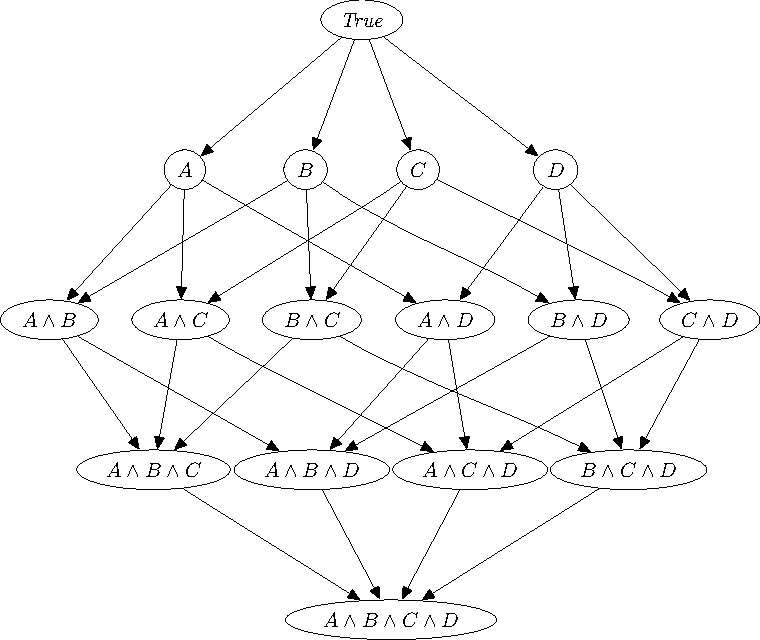
\includegraphics[width=8cm]{gfx/example_conjunctive_hypothesis_space}
\caption[An example of a conjunctive hypothesis space.]{An example of
  a conjunctive hypothesis space.}
\label{figure:example_conjunctive_hypothesis_space}
\end{figure}


\section{leftovers...}

\section{Causal Knowledge}

Now that a separate temporal sequence for each reflective layer has
been defined, this factual grounded knowledge can be abstracted into
hypothetical causal models that are useful for planning toward goals
in a counterfactual future.



{\mbox{\autoref{figure:example_causal_knowledge}}} shows an example of
causal knowledge.
\begin{figure}
\center
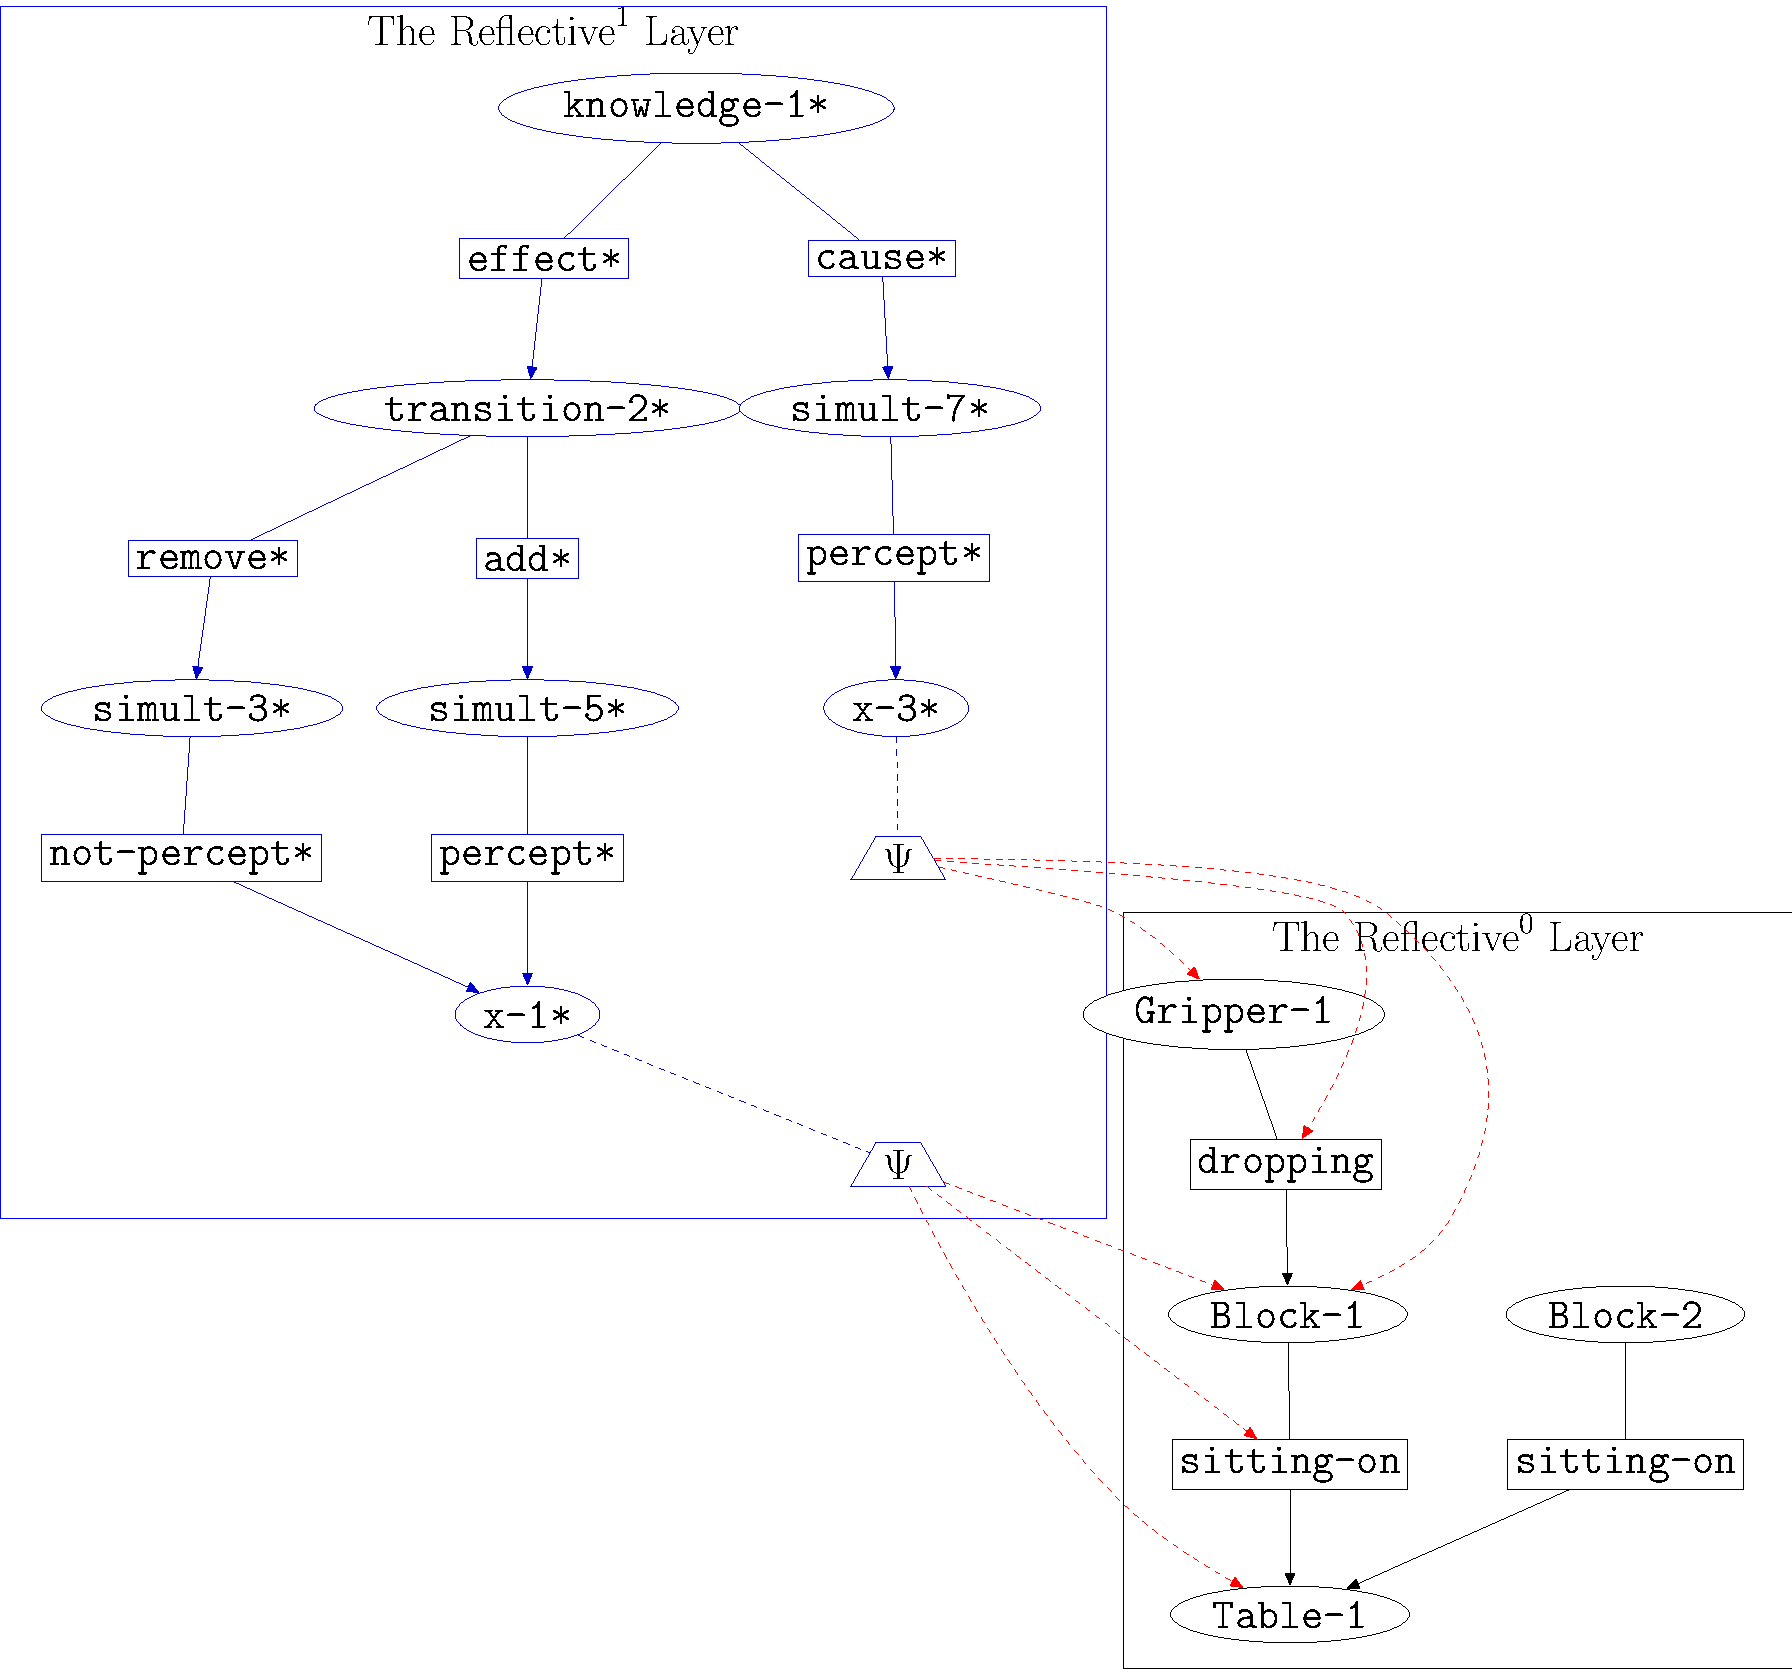
\includegraphics[width=12cm]{gfx/example_causal_knowledge}
\caption[An example of a causal knowledge.]{An example of causal
  knowledge, $\text{\tt{knowledge}}_1^*$, where the simultaneity,
  $\text{\tt{simult}}_7^*$, is known to be the cause of the
  transframe, $\text{\tt{transition}}_2^*$.  Negative perceptions are
  omitted here for to reduce visual clutter.}
\label{figure:example_causal_knowledge}
\end{figure}

\section{Representing Causal Hypotheses}

{\mbox{\autoref{figure:example_causal_hypothesis}}} shows an example
of a causal hypothesis, $h_1^*$, where the simultaneity,
$\text{\tt{simult}}_7^*$, is hypothesized to be the cause of the
transframe, $\text{\tt{transframe}}_2^*$.  In other words, the gripper
dropping the block causes the block to be sitting on the table.
\begin{figure}
\center
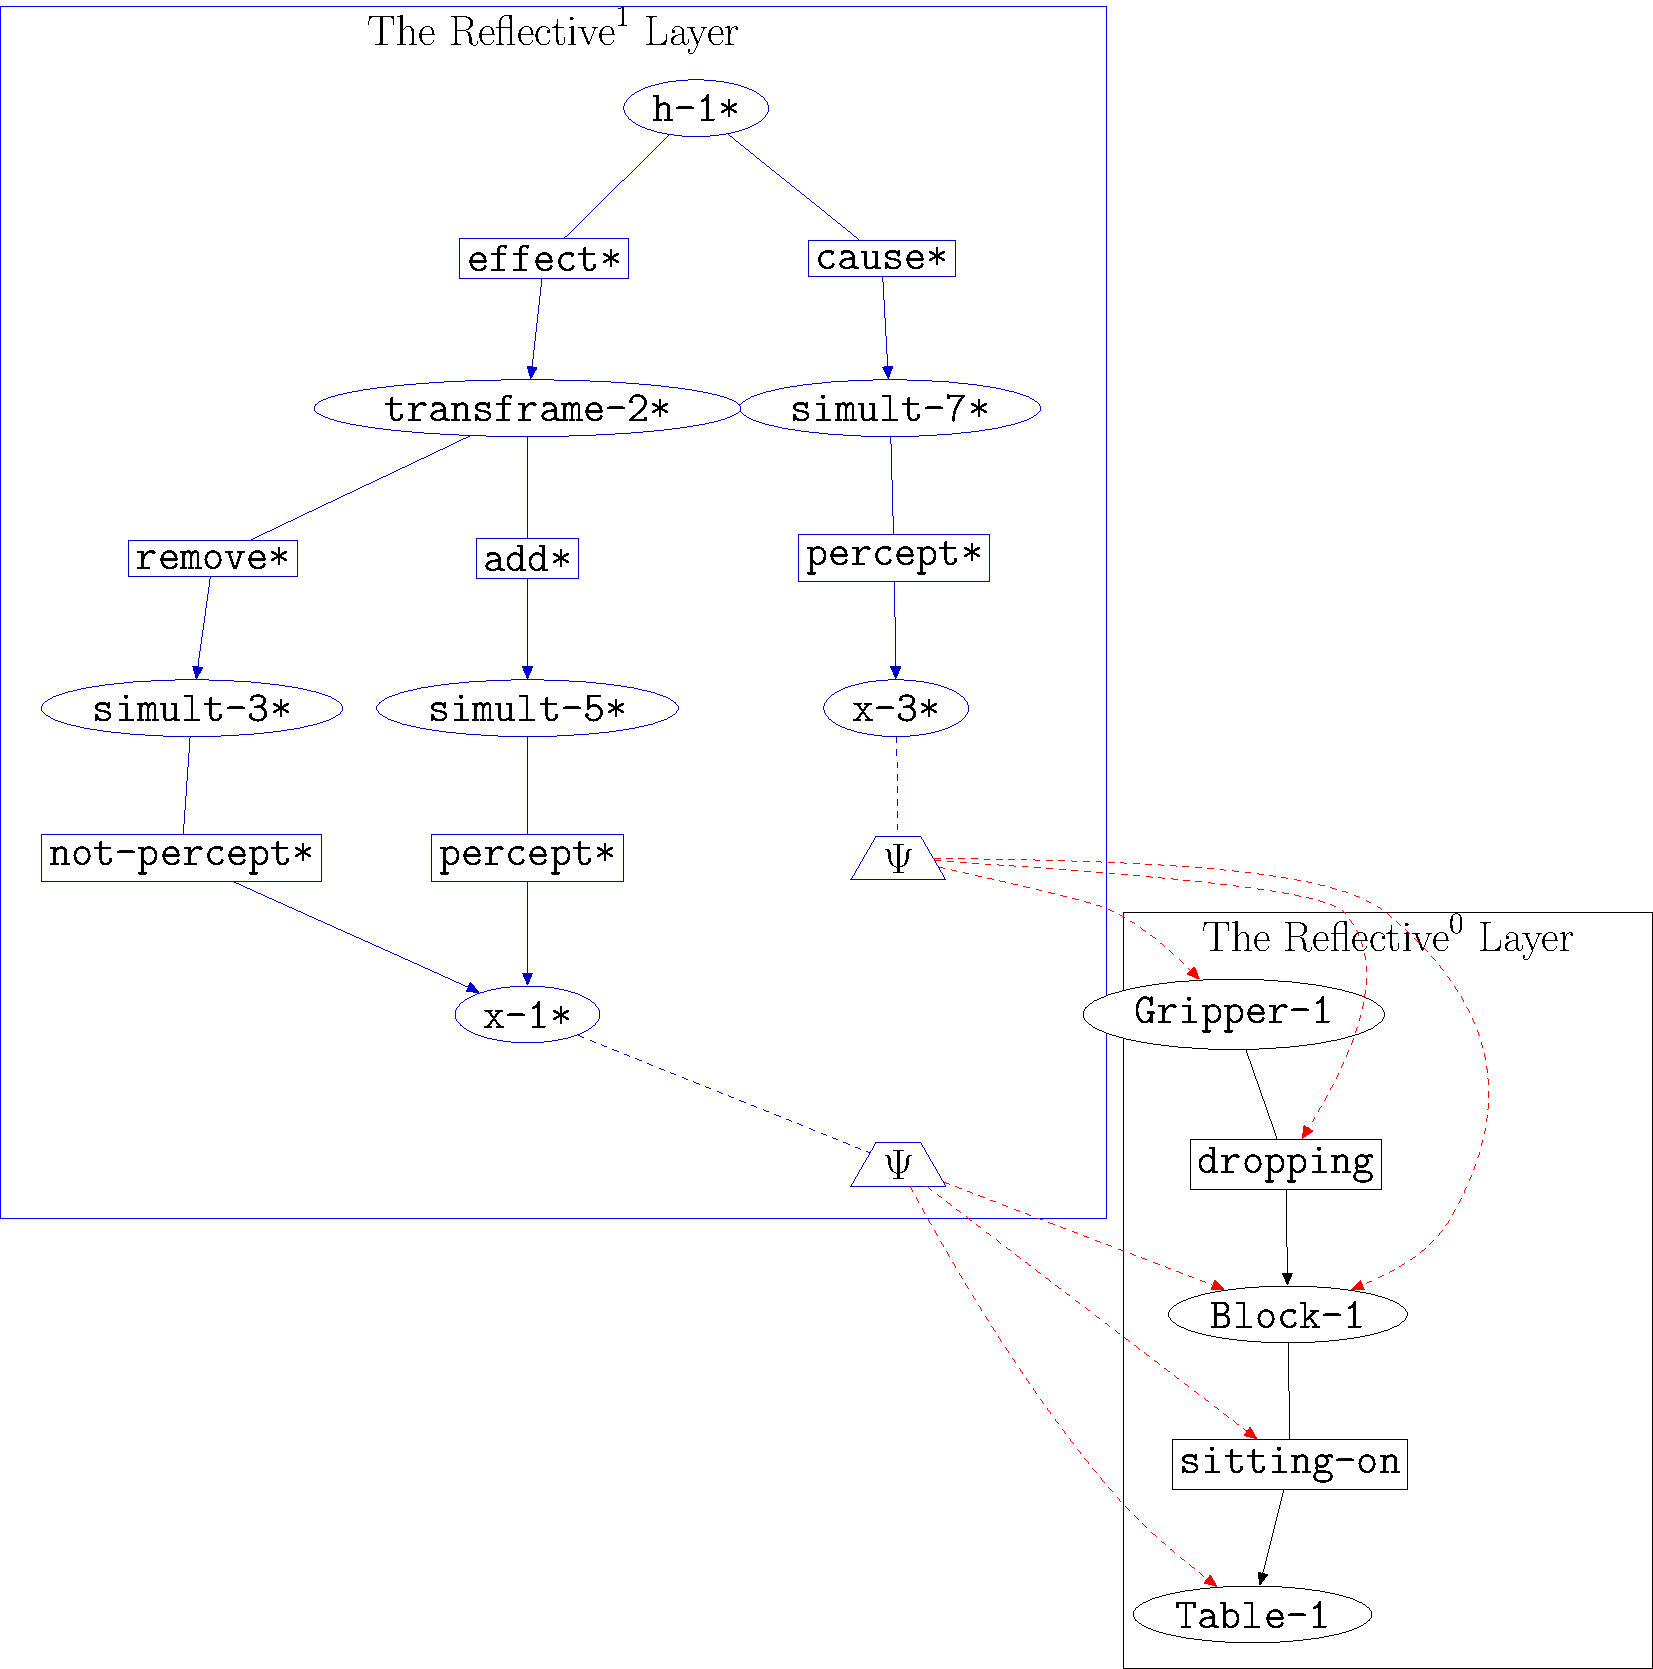
\includegraphics[width=8cm]{gfx/example_causal_hypothesis}
\caption[An example of a causal hypothesis.]{An example of a causal
  hypothesis, $h_1^*$, where the simultaneity,
  $\text{\tt{simult}}_7^*$, is hypothesized to be the cause of the
  transframe, $\text{\tt{transframe}}_2^*$.  In other words, the
  gripper dropping the block causes the block to be sitting on the
  table.}
\label{figure:example_causal_hypothesis}
\end{figure}

\section{Composing Plans from Hypotheses}

